\chapter{Introduction}\label{intro}
\section{Person re-identification}
In recent years, with the increasing demand for public safety and security, the network of video surveillance cameras are proliferating in both public and private areas. In order to reduce the number of crimes and terror attacks, and to provide a safer and secure environment, it is necessary to improve the current state of the surveillance system by implementing computer vision-based algorithms to automatically recognize a suspicious person. However, unfortunately, existing surveillance systems only have the capacity to capture and store the video leaving the task of detecting abnormal events in human operators. Therefore, there has been a great effort by the computer vision and artificial intelligence (\gls{ai}) communities to develop an intelligent video surveillance system capable of real-time monitoring and alerting. Person re-identification (\gls{reid}), a fundamental task of intelligent video surveillance systems, refers to recognizing the same person across a network of cameras with non-overlapping fields of view from given single or multiple images. Besides security and surveillance, it is needed for a lot of applications such as authentication, human-computer interaction, cross-camera person tracking, human behavior and activity analysis. 

A basic person re-identification scenario can be shown in Figure~\ref{fig:person_reid}. In a surveillance system person \gls{reid} helps us to know when and where a person appears with respect to a given camera, and in a network of multiple cameras, it potentially allows us to estimate his/her trajectory over a short period of time. 

However, person \gls{reid} remains an open problem to be addressed in real-time surveillance due to the large variation in camera view angle, pose and illumination variation, partially or complete occlusions, and subject intrinsic variations. However, among these, the viewpoint variation is one of the most challenging problems which simultaneously creates the intra-class variation and the inter-class confusion.


\begin{figure}
	\centering {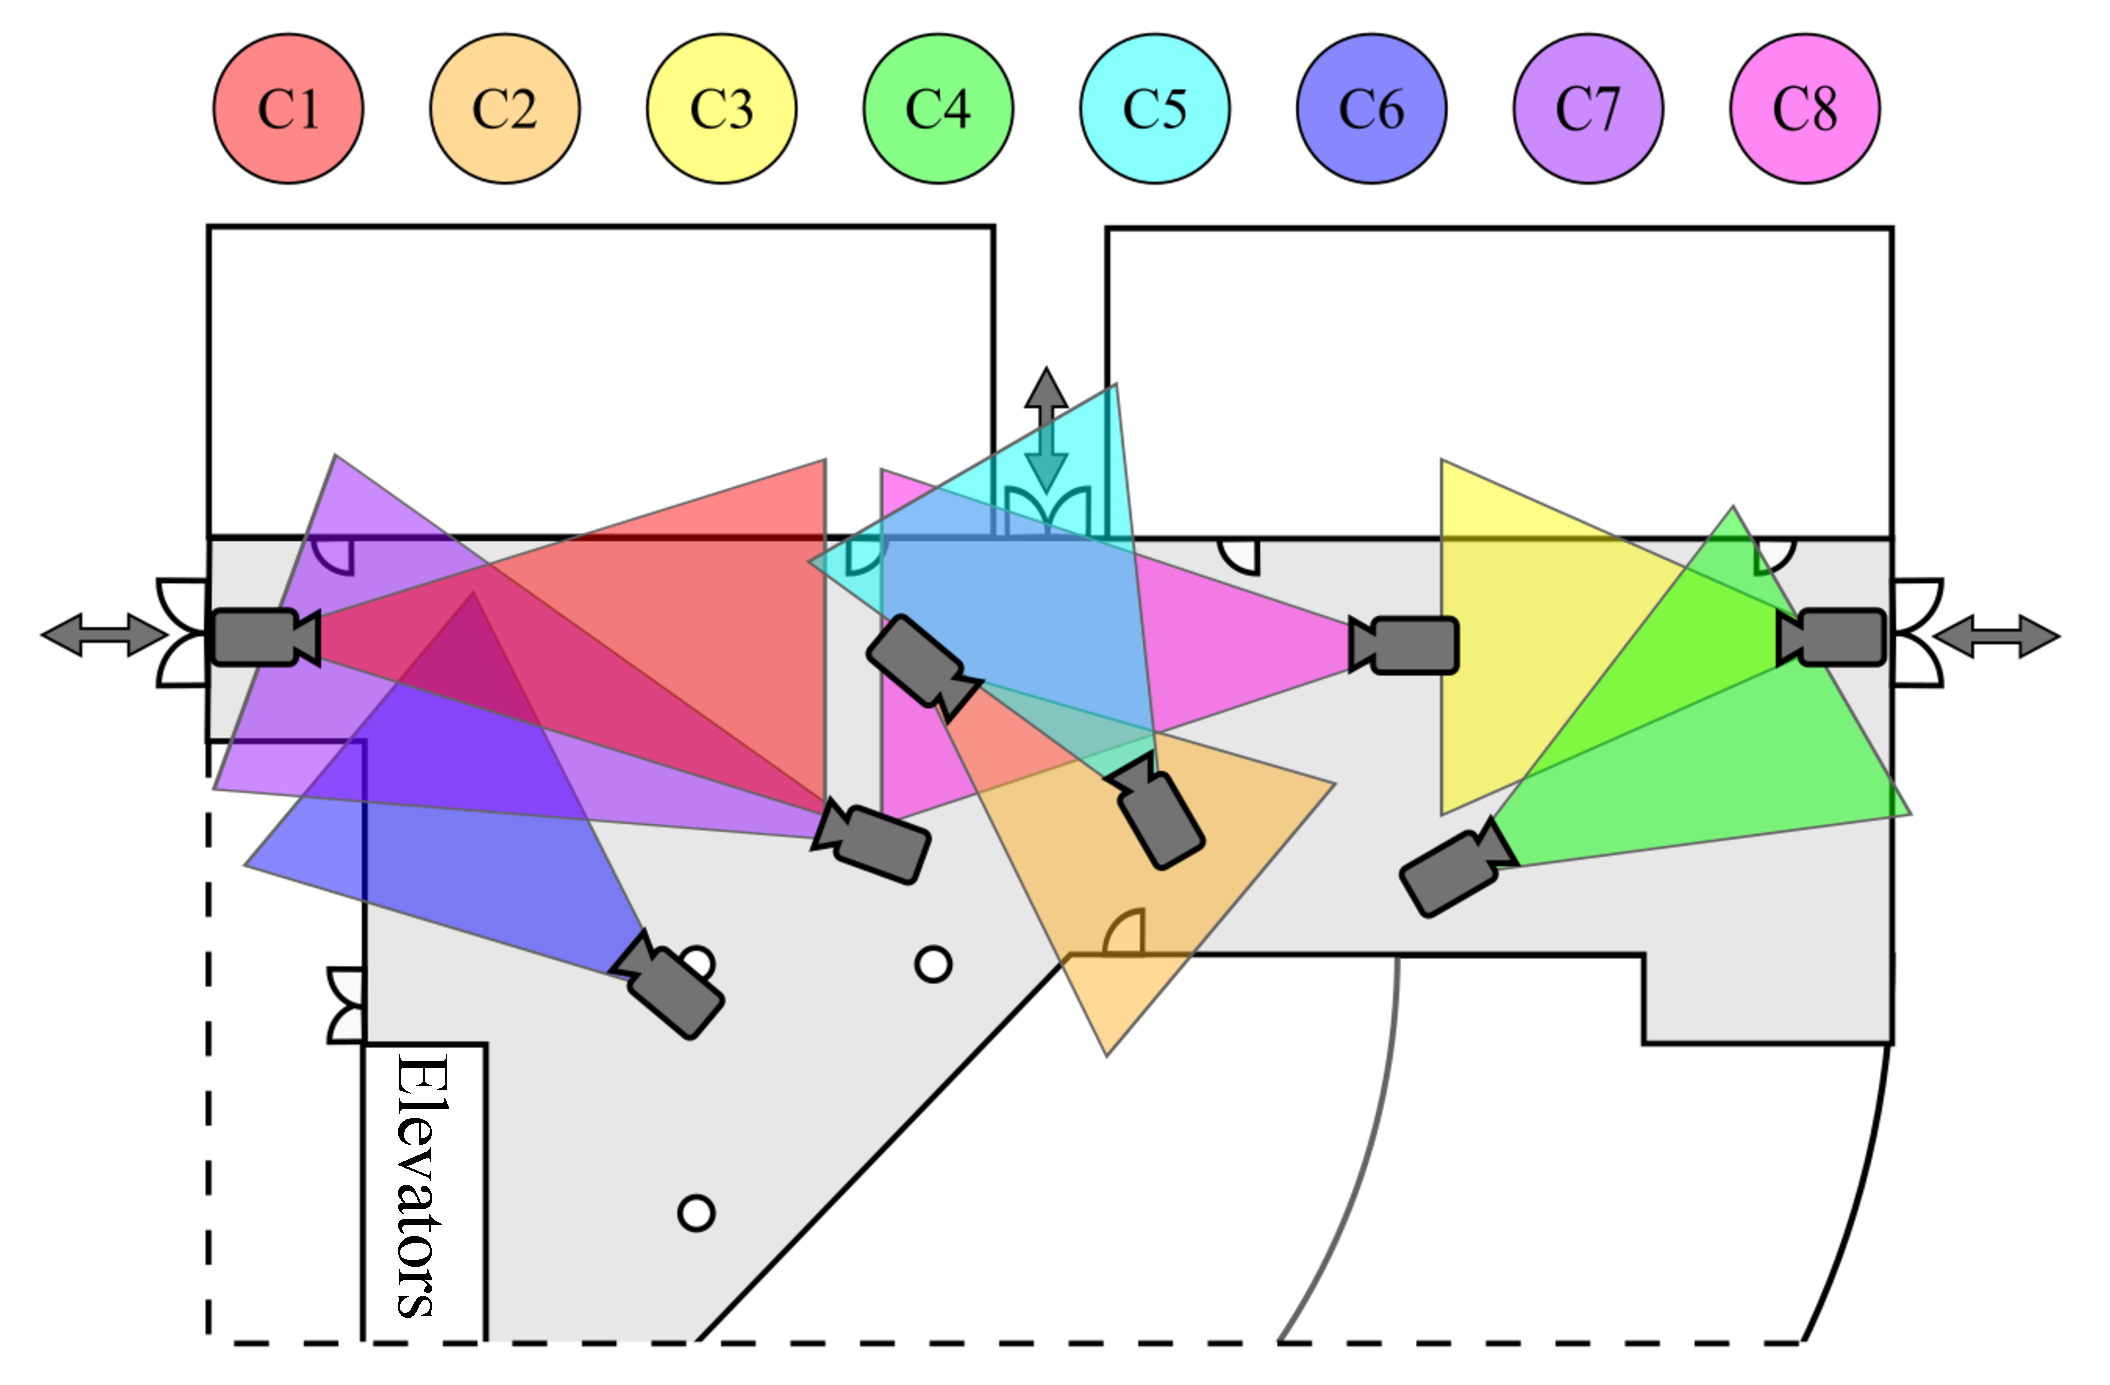
\includegraphics[width=0.7\textwidth]{figures/person_reid.eps}}
	\caption[A basic topology of person re-identification in a multi-camera network environment]
	{A basic topology of person re-identification in a multi-camera network environment. A person should have the same label when walking through the surveillance camera network. \label{fig:person_reid}}
\end{figure}


\section{Gait Recognition}
\subsection{Definition}
Biometrics refers to the automatic identification or authentication of people by analyzing their physiological and behavioral characteristics. Physiological biometrics is related to the shape of body parts such as the face, fingerprints, shape of the hand, iris, retina, etc., which are not subject to change due to aging. It is now used as the most stable means for authenticating and identifying people in a reliable way. However, for efficient and accurate authentication, these traits require cooperation from the subject along with a comprehensive controlled environmental setup. Hence, these traits are not useful in surveillance systems. Behavioral biometrics such as signatures, gestures, gait, and voice, etc., is related to a person’s behavior. But, these traits are more prone to change depending on factors such as aging, injuries, or even mood. 

\textit{Gait} can be defined as the coordinated, cyclic combination of movements that result in human locomotion~\cite{Boyd_05}. The movements of gait are coordinated in the sense that they must occur with a specific temporal pattern and cyclic in nature since a walker cycles between steps with alternating feet. It is both the coordinated and cyclic nature of the motion that makes gait a unique phenomenon to each individual. Although these movements follow the same basic bipedal pattern for all humans, they seem to vary from one person to another considerably in their relative timing and magnitudes~\cite{Benabdelkader_02}.

\textit{Gait recognition} is a behavioral biometric modality that identifies a person based on his/her gait pattern. Among the behavioral biometrics cues, gait is very relevant to person \gls{reid} in surveillance networks. It is the most prevalent human movement in typical surveillance spaces. 


\subsection{Advantages}
In contrast to other biometrics such as face and fingerprint, gait has several attractive properties. For example, it is a non-invasive technique for identifying an individual which is hard to copy. It doesn't require any cooperation or awareness of the subject. Another unique advantage of gait as a biometric is that it offers recognition at a greater distance with simple instrument. Additionally, recognition can also be done reliably at low-resolution images. Other biometrics may not provide the required accuracy under these conditions. Due to these potential advantages, gait has attracted significant attention in recent years. Consequently, gait biometric signature is now considered as the only likely identification technology suitable for access control, covert video surveillance, criminal investigation, and forensic analysis where the method is not vulnerable to spoofing attacks and signature forgery. In addition to the authentication applications, gait analysis can also be used in medical applications for abnormality detection, Parkinson's disease~\cite{Michele_17}, and Chronic disease~\cite{Juen_14}.


\begin{figure}
	\centering {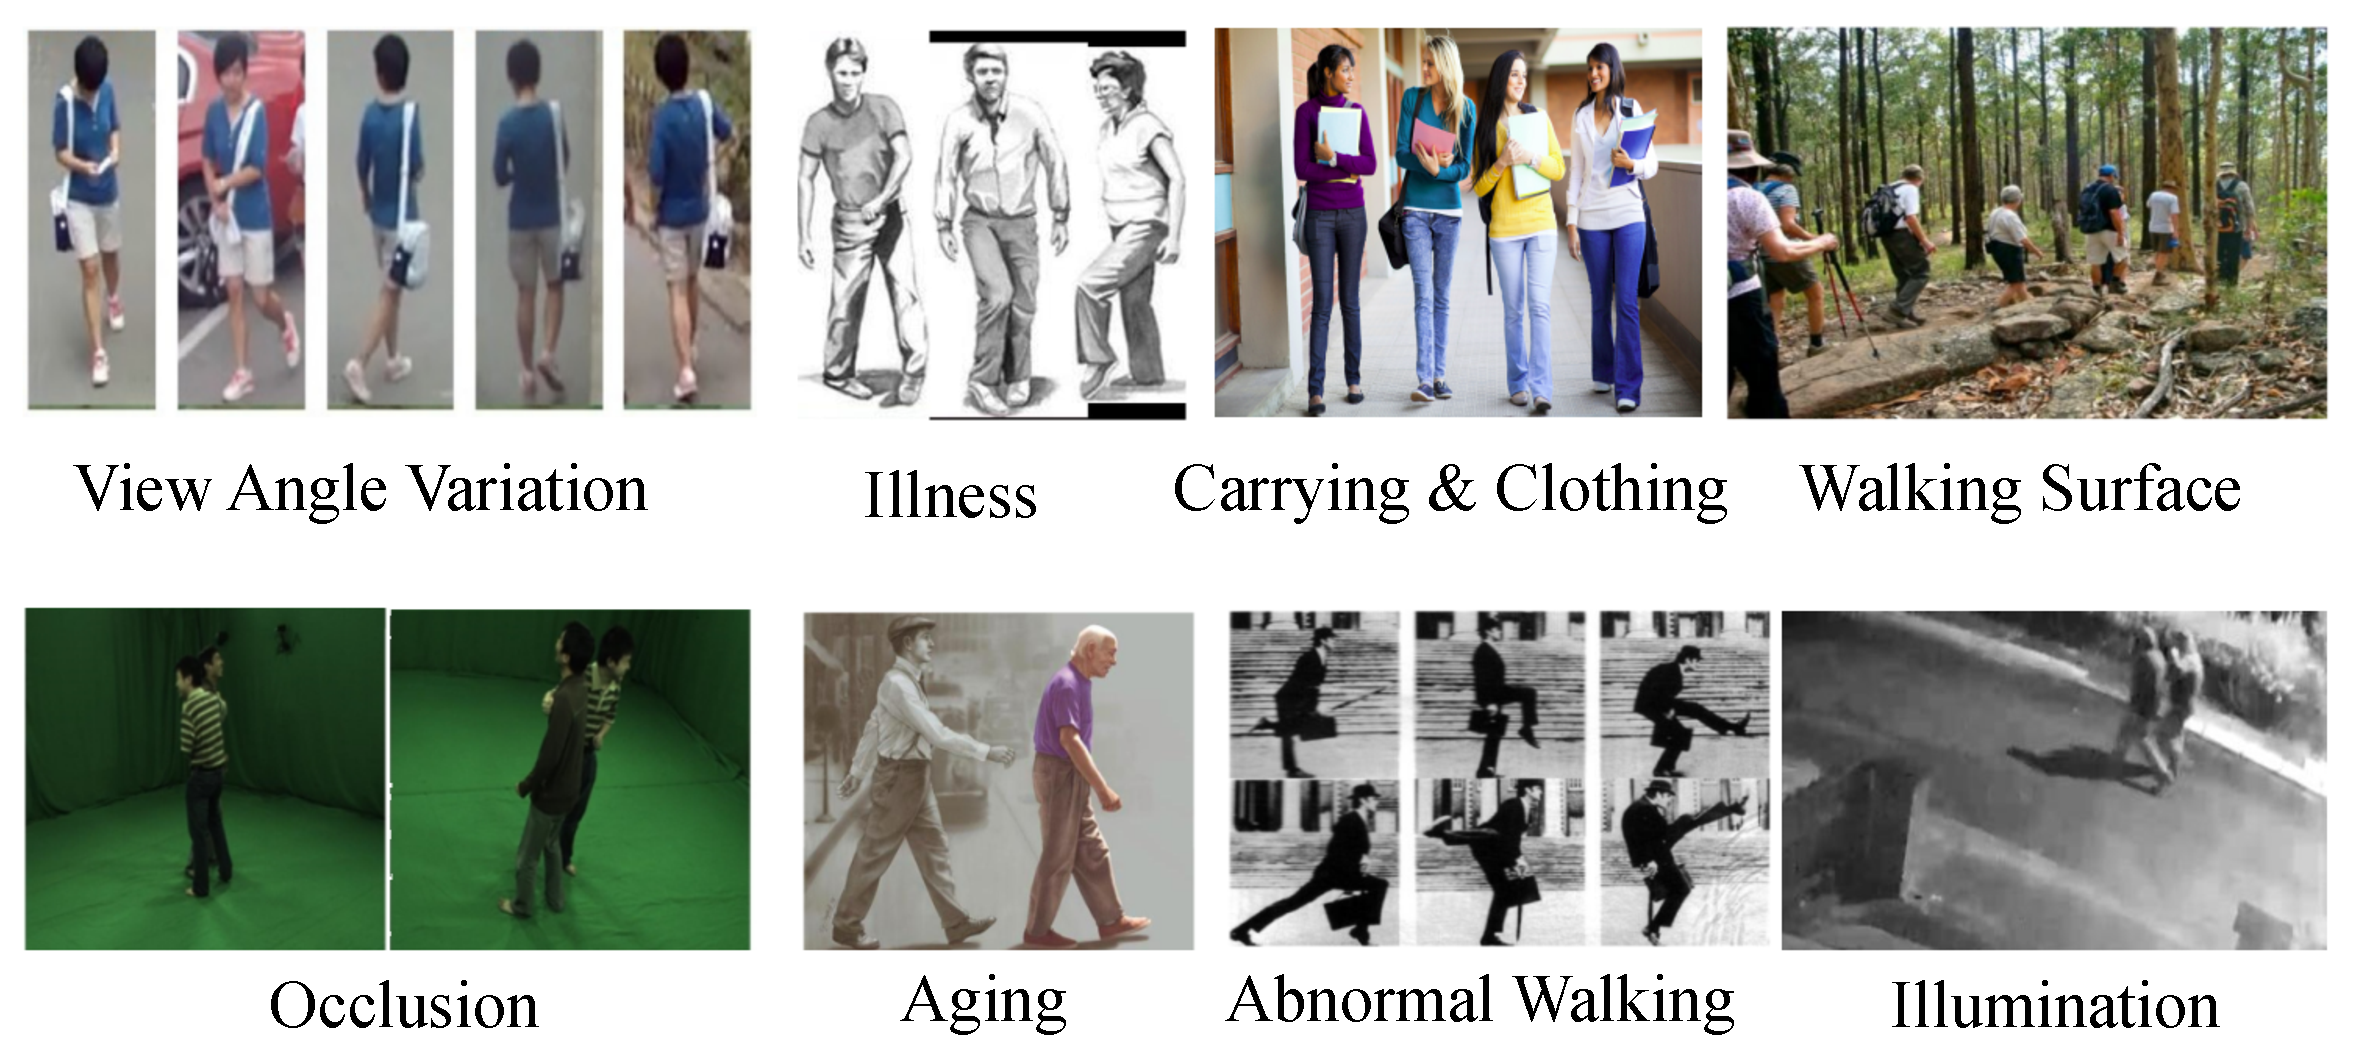
\includegraphics[width=\textwidth]{figures/gait_challenges.eps}}
	\caption[A basic topology of person re-identification in a multi-camera network environment]
	{Common challenges in gait recognition \label{fig:gait_challenges}}
\end{figure}

\subsection{Challenges}
It has been observed that some recent gait recognition algorithms have achieved $100\%$ classification accuracy under controlled environmental setup. However, these results significantly degrade in real-world scenarios due to the presence of various challenging factors. Due to these covariate factors gait recognition in real-world multi-camera environment remains an open research problem which yet prevent it to be employed in public places for security surveillance-based applications. 

Gait recognition is highly affected by the change in environment such as variations in view angle, illumination, and walking surface as well as different intraclass variations such as variation in clothing and carrying condition. Some of the challenging factors and their effects are explained in following.
\begin{itemize}
	\item \textbf{View angle variation}: Since with the variation of camera position the distance between the subject and the camera as well as the walking direction of the subject are varying, different sizes or shapes of the subject can be observed in different viewing angles. Moreover, one view can contain partial information of subject's body pose. Even some the body parts of the subject are not visible in one view angle, but could be visible in another view angle. Furthermore, in same view angle different people's shape may look more similar compare to the shape of same subject under different view angle. 
	
	\item \textbf{Partial occlusion}: Sometimes subjects are partially or completely occluded by overlapping with other people or objects. 
	
	\item \textbf{Low resolution}: Surveillance cameras are usually installed in high places on walls which are far away from the subject. Therefore, the captured videos are in low resolution which often cause inaccurate body pose estimation.
	
	\item \textbf{Clothing or carrying variation}: The subject may appear with different clothing and carrying object in different camera views. For example, subject may wear a coat or take the backpack in hand from back.
	
	\item \textbf{Illumination variation}: In a network of multiple camera illumination condition can vary. Therefore, the same subject can have a color difference on the appearance under different lighting conditions. 
\end{itemize}

Some of the examples images illustrating these challenges are shown in Figure~\ref{fig:gait_challenges}. So, these challenges are needed to be addressed for robust gait recognition.



\section{Problem Definition}
Gait based person re-identification in surveillance is a problem of recognizing individuals based on their gait pattern at different times and locations from a network of interconnected cameras, without overlapping views. However, the presence of various covariate factors make the problem very challenging. Although a multitude of researches have been done in recent years, it remains an open problem and many of its aspects have yet to be addressed. This research aims to 
build a robust algorithm in order address these challenges. It also investigate ways to incorporate the multi-view data to solve the problem of view-dependency in multi-camera network.

There are fundamental differences between the gait-based recognition and person \gls{reid} in general scenarios. For general person \gls{reid}, the operator has the control over most of the acquisition factors, e.g., camera viewpoint, the number of persons in the image, chance of occlusion, subject pose, and illumination, etc. However, in person \gls{reid} under real-world surveillance most of these conditions are uncontrolled, e.g., changes in viewpoint and illumination over a large number of different cameras, no control on the number of people and possible occlusions, also subjects’ varying walking direction. Therefore, due to the unconstrained nature of the problem, gait recognition algorithms are now considered as a potential biometric tool to solve person \gls{reid} in real-world video-based surveillance applications~\cite{Lee_14}.




\section{Objectives of the Thesis}
The objective of this thesis is to design a gait recognition system for person re-identification in a multi surveillance camera environment. To achieve this objective, we have identified the following specific aims.

\begin{itemize}
\item To design a novel low-dimensional gait feature descriptor based on the pose information of the people detected in the gait videos To design a mechanism to detect people in gait videos and determine their pose sequences. 

\item To develop a robust pose based gait recognition algorithm using recurrent neural network (RNN), which will be invariant to factors like viewing angle, clothing, presence of bags, etc.

\item To identify people across a set of interconnected surveillance cameras.

\item To compare the results with state-of-the-art methods.
\end{itemize}



\section{Overview of the Thesis}
Modern deep learning-based algorithms have recently gained increasing popularity while achieving outstanding performance in many computer vision tasks such as video classification~\cite{karpathy_14}, pose estimation~\cite{Cao_19}, and action recognition~\cite{Song_17, Du_15}, etc. A recurrent neural network (\gls{rnn}s), a type of artificial neural network, where connections between nodes form a directed graph along a temporal sequence. \gls{rnn}s have also achieved a promising performance in many sequence labeling tasks. The reason behind their effectiveness for sequence-based tasks lies in their ability to capture long-range dependencies in a temporal context from a sequence. \gls{rnn}s have been successfully employed to achieve state-of-the-art results in many vision-based tasks like image captioning~\cite{Mao_15} and action recognition~\cite{Song_17, Du_15}. Furthermore, advancement on human body pose estimation can significantly assist in accurately modeling different human body parts required for gait recognition. 

In this thesis, we propose a model-based gait recognition method where we consider human 2D pose information for our effective gait feature as human pose is proven not to be dependent on people's body appearance, and is invariant to change of clothing and carrying conditions. Additionally, as gait can be considered a time series of walking postures, body pose information has a powerful capacity to capture the temporal pattern of gait. Therefore, the proposed method will be less affected by the variation of covariate factors. It is also worth mentioning that, in this work, we didn't use 3D pose data as our gait feature: firstly, computing 3D poses is computationally expensive, and secondly, most of the 3D pose estimation algorithms recover 3D pose from 2D RGB images which often require multiple views, and hence multiple cameras, rendering the technique unsuitable for surveillance. Again, recovering 3D pose from a single RGB image is an ill-posed problem and often causes large pose estimation errors. 

Compared to other gait covariates, view is the most important factor which severely affects gait recognition performance. To handle view variation efficiently, gait algorithms have generally been studied under three experimental setups: single-view, multi-view, and cross-view setup. In single-view gait recognition, both probe and gallery gaits are kept within same view angle, wherein cross-view gait recognition, the probe and gallery gaits are kept in different views; and in multi-view gait recognition, multiple views of gallery gaits are combined to recognize a probe gait under a specific view.

Thus, the main idea of our proposed method is to develop a pose-based recurrent neural network for robust gait recognition by modeling the temporal dynamics associated with human gait. Most of the descriptors proposed in the literature for gait recognition often lead to a high dimensional feature space which are computationally expensive to map. In this research, we designed a lower-dimensional spatio-temporal feature descriptor from 2D pose estimation for improved performance at a reduced computational cost. Our gait descriptor is a concatenation of four different types of feature vector. For multi-view gait recognition, we also propose a two-stage network in which we first determine the walking direction, i.e., the view angle of the camera using a 3D convolutional network and later identify the subject using proposed \gls{rnn}-based temporal network trained on that particular angle. 

We demonstrate the effectiveness of our proposed method through extensive experiments on two public benchmark datasets: the CASIA A and CASIA B gait dataset~\cite{Yu_06}. Our method achieved state-of-the-art performance on these two challenging gait datasets in both single-view and cross-view recognition, providing better results as compared to other state-of-the-art methods. Besides that our method is far simpler and efficient in terms of time and space compared to other methods proposed in the literature. Again, in multi-view gait recognition, our method outperforms other architecture at a significant margin. 



\section{Contributions}
Original contributions resulting from the research presented in this thesis are fourfold:
\begin{itemize}
\item We introduce a novel low-dimensional discriminative gait feature vector from 2D body pose information which is invariant to covariate factors and achieved comparable performance to the methods which require to calculate gait energy image (GEI) or expensive 3D poses for gait descriptors.

\item We design a novel \gls{rnn} network with \gls{gru} architecture and devise several strategies to effectively train the network for robust gait recognition. 

\item We also propose a two-stage network for multi-view gait recognition in which we first identify the walking direction using a 3D convolutional network and then performs subject recognition using a temporal network trained on that particular angle.

\item The proposed pose-based \gls{rnn} network achieves the best results on two challenging benchmark datasets CASIA A and CASIA B by outperforming other prevailing methods in single-view and multi-view gait recognition at a significant margin.
\end{itemize}


\section{Thesis Outline} 
In the rest of this thesis, we present the details of our approach for robust gait recognition. Here
\begin{itemize}
\item \textbf{Chapter~\ref{ch:literature_review}} provides a survey of existing gait recognition techniques and evaluates them for their strengths and limitations.
\item \textbf{Chapter~\ref{ch:methodology}} describes the proposed framework used in this thesis with all required preprocessing, modeling and network architecture for both single-view and multi-view gait recognition. It also presents the training strategies of these models with complete implementation details.

\item \textbf{Chapter~\ref{ch:experimental_result}} gives the experimental evaluation of the proposed framework on publicly available datasets, namely CASIA A and CASIA B dataset. It also compare our results with other state-of-the gait recognition algorithms in different experimental setup on these datasets and discusses them. 

\item \textbf{Chapter~\ref{ch:conclusion}} concludes this work with a summary over the different contributions and presents some perspectives about possible future research directions.
\end{itemize}


